
\section{2008}

\subsection{January 2008}

\vspace{.15in}\noindent{\bf January 16, 2008}

Today I started recasting all my JOD documentation as \LaTeXe.  For the
last few months I've been  rewriting my word based
JOD documentation using \emph{Google's} online word processor.  There
are somethings I like about this tool.  
\begin{enumerate}
	\item The documents are online.
	\item Document source is a variant of HTML.
	\item The tool is easy to use.
	\item You can export your documents in a number of handy formats.
\end{enumerate}
This is all good but I've reached the point where the limitations
of the tool are getting in my way.  

One of the main goals of my JOD documentation efforts is to produce
and maintain a single primary source.  All forms of documentation,
PDF, online, paper must be generated automatically from this
single source \emph{without vast headaches.}  The Google tool just isn't
up to this. 

I was planning to write some J code to convert the quasi-HTML generated
by the Google tool to \LaTeXe\ but I quickly discovered this is just to much work!

My new plan is:
\begin{enumerate}
	\item Write the JOD document using \LaTeXe.
	\item Convert the \LaTeXe\  to HTML using \verb?latex2html?.
	\item Write some J code to split up the generated HTML for \texttt{jodhelp}.
\end{enumerate}
This will still be a lot of work.  \verb?latex2html? comes from the Perl/Linux world
and getting it working under Windows will require some tweaks.  It has been
done so I won't be breaking new ground --- not gonna do that anymore for documentation.

\subsection{February 2008}

\vspace{.15in}\noindent{\bf February 1, 2008}

I have been playing with Oleb's \href{http://www.graphviz.org}{\emph{graphviz}} addon. 
Figure~\ref{eps:joddot} on page~\pageref{eps:joddot} displays the current class structure of
the JOD system.  


\begin{figure}[htbp]
  \centering
  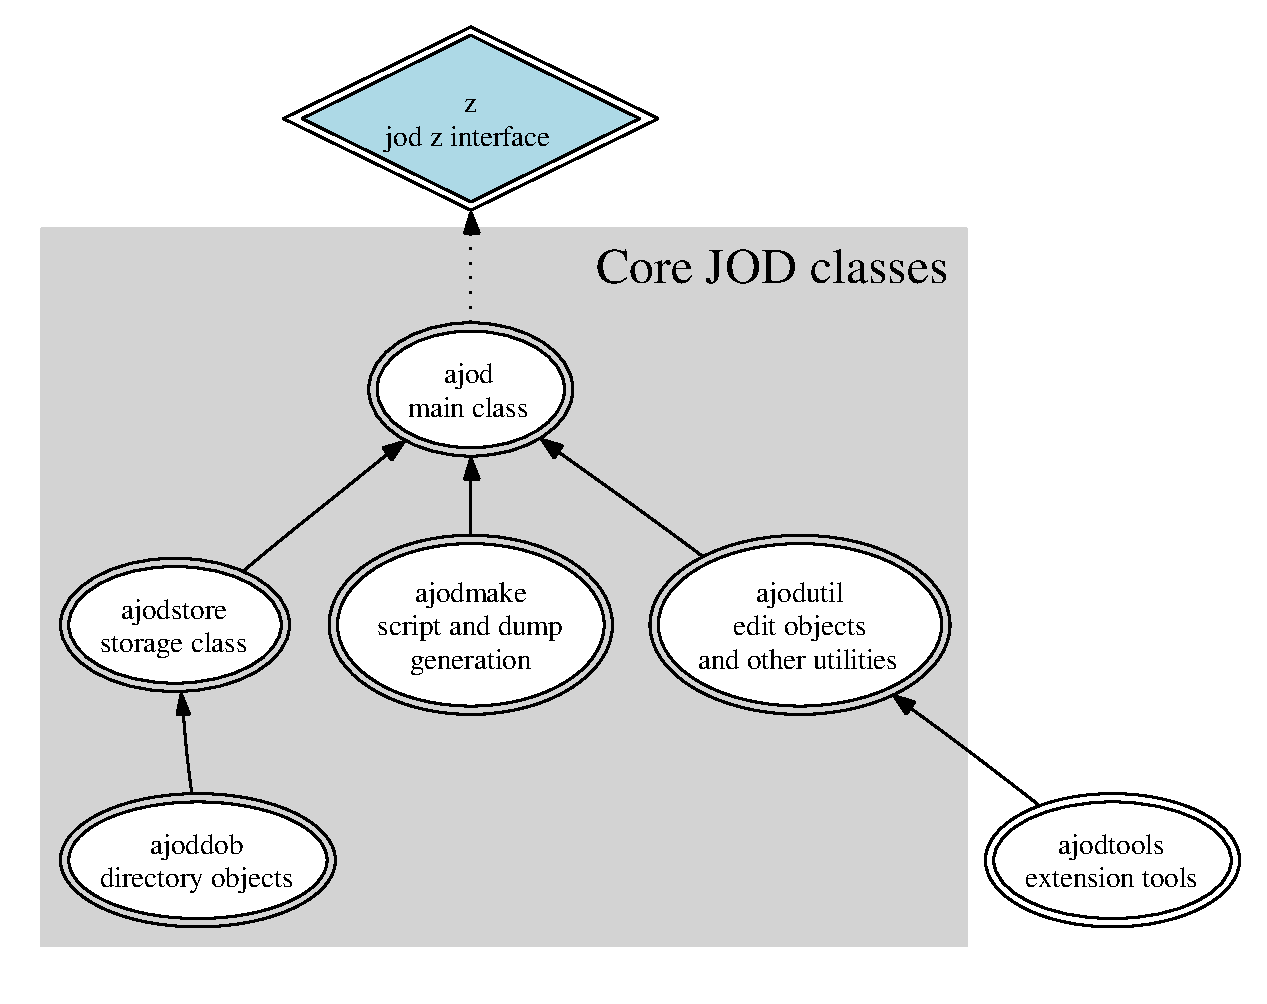
\includegraphics[width=\textwidth]{joddot}
  \caption[JOD Classes]{JOD Class digraph.}
  \label{eps:joddot}
\end{figure}


\vspace{.15in}\noindent{\bf February 5, 2008}

Yesterday I had a colonoscopy and today I'm preparing to pay both US and Canadian income
taxes.  The colonoscopy affirmed there is room up there for the incoming tax broom handle.
On the JOD front I worked on converting JOD Google documents to \LaTeXe\.  I am aiming to
produce a single definitive PDF JOD document that describes the system.